%The paper size, font size and document type are defined in the following
\documentclass[a4paper,12pt]{article}

%Uncomment the following line, if you write in Finnish (special characters)
%\usepackage[utf8]{inputenc}

%\usepackage[finnish]{babel}
\usepackage[english]{babel}

\usepackage{graphicx}
\usepackage[parfill]{parskip}

%useful special symbols:
\usepackage{amssymb}
\usepackage{latexsym}
\usepackage{amsmath}
\usepackage{amsthm}

\usepackage[toc,page]{appendix}

%a useful package if you write url addresses:
\usepackage{url}
\usepackage{hyperref}

%a package for figures:
% \usepackage[dvips]{color}
\usepackage{epsfig}

%a package for rotated figures and tables:
\usepackage{rotating}

\usepackage{biblatex}

\usepackage{listings} % For including code
\usepackage{xcolor}   % For defining code colors

%% Define custom colors for the code
\definecolor{codegreen}{rgb}{0,0.6,0}
\definecolor{codegray}{rgb}{0.5,0.5,0.5}
\definecolor{codepurple}{rgb}{0.58,0,0.82}
\definecolor{backcolour}{rgb}{0.95,0.95,0.92}

% Define Python code style
\lstdefinestyle{mystyle}{
    backgroundcolor=\color{backcolour},   
    commentstyle=\color{codegreen},
    keywordstyle=\color{magenta},
    numberstyle=\tiny\color{codegray},
    stringstyle=\color{codepurple},
    basicstyle=\ttfamily\footnotesize,
    breakatwhitespace=false,         
    breaklines=true,                 
    captionpos=b,                    
    keepspaces=true,                 
    numbers=left,                    
    numbersep=5pt,                  
    showspaces=false,                
    showstringspaces=false,
    showtabs=false,                  
    tabsize=4
}

% Apply the style to Python listings
\lstset{style=mystyle}

\addbibresource{references.bib}

\graphicspath{ {./figures/} }

%if you want smaller page margins, uncomment and adjust the following
%\textheight=24.3cm
%\topmargin=-1.8cm
%\textwidth=16.7cm
%\oddsidemargin=-0.3cm
%\evensidemargin=0.0cm


%Create your own environments
\newtheorem{definition}{Definition}
\newtheorem{example}{Example}
\newtheorem{theorem}{Theorem}

%and useful macrosfor faster writing (benefit: you can change the notations 
%later, e.g., two possible notations for your vector x)
\newcommand{\Mmatr}{\ensuremath{\mathbf{M}}}
\newcommand{\xvec}{\ensuremath{\overline{x}}}
\newcommand{\xvecII}{\ensuremath{\mathbf{x}}} %alternative def
\newcommand{\Xset}{\ensuremath{\mathbf{X}}}
\newcommand{\fr}{\ensuremath{\mathit{fr}}} %just neater typing

%If you want to remove the space before paragraphs uncomment the following.
%Remember then to leave an empty line between paragraphs! 
%\setlength{\parindent}{0pt}


\title{MDM-2024 Homework 2}
\author{Cuong Nguyen (101559968), Petteri Raita (909635),\\and Raihan Gafur (101555441)}

%Uncomment the following, if you don't want the date to be printed
%\date{}

\begin{document}

\maketitle
\tableofcontents
\newpage

\listoffigures
\newpage

% include tex files of sections here, e.g.
% \input{section1.tex}
% \input{section2.tex}
\section{Methods}
In this experiment, Python was used as the primary programming language, utilizing the
libraries \texttt{numpy} for numerical computations and \texttt{matplotlib} for plotting
and visualization. The randomization interval for generating the data points was the
half-open interval \([0,1[\), excluding the origin. The Lp norms were computed using
a custom function:

\lstinputlisting[language=Python]{code/lp_norm.ipynb}

which supported a range of \(p\) values, including p = 0.5, 0.8, 1, 1.3, 1.5, 1.7, 1.9,
1.95, 2, 5, and \(\infty\). For each experiment, \(q = 100\) data sets, each containing
\(N = 100\) points, were generated across various dimensions \((k = 2, 3, 4, 5, 10, 20,
30, 40, 50, 60, 70, 80, 90, 100, 150, 200, 250, 300)\).

% Question 3 Petteri
\section{Results}
\subsection{NMI}

The different clusterings were evaluated for all the different feature combinations, linkage methods, and number of clusters. The scoring for each individual combination of features was based on the NMI of the cluster with the real labels (the biological groupings). However, the best NMI value included 12 clusters of which there were one or more singleton clusters. Since NMI is excessively influenced by the singleton clusters, those were filtered out.

As a result, the highest NMI score for a clustering was 0.727. This score was provided by a combination of 11 cluster with the selected features being AR, wload, WSI, and the back color. The clustering used a complete linkage. Comparing this clustering to the other top candidates in terms of NMI, the common features were very much the same as with the chosen clustering. Only a few combinations dropped the AR or the wload. Out of the best 10 combinations, none used BMI as a feature. This is indicative of the statistically low information provided by the BMI feature. The number of clusters was between 9 and 12, which is a relatively small difference.

\begin{figure*}[ht!]
    \centering
    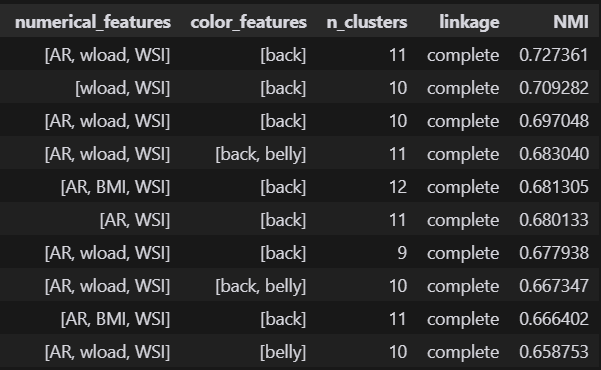
\includegraphics[width=0.8\textwidth,height=\textheight,keepaspectratio]
    {nmi_scores.png}
    \caption{\emph{NMI Values}}\label{fig:top_10_NMI_scores}
\end{figure*}



% Mutual Information (MI)
The normalized mutual information score was calculated through the Sklearn library, which uses the following formula for the calculation of the mutual information score. The normalization of the score uses the entropies of the classes and labels to normalize the MI value to fall between 0 and 1.


The Mutual Information is a measure of the similarity between a cluster and the biological grouping. In the code, the true labels for NMI score were the 'group' column of the data. The predicted labels were found through fitting the clustering method to the data.

% Where $|U_i|$ is the number of the samples in cluster $U_i$ and $|V_j|$ is the number of the samples in cluster $V_j$, the Mutual Information between clusterings $U$ and $V$ is given as:

\[
    MI(U, V) = \sum_{i=1}^{|U|} \sum_{j=1}^{|V|} \frac{|U_i \cap V_j|}{N} \log \left( \frac{N |U_i \cap V_j|}{|U_i| |V_j|} \right)
\]



\subsection{Analysis of the cluster contents}



Comparing the clustering results with the actual groups and flying types, it is evident that there are clear common features among the clusters. For example, the cluster contents align well with the flying types, notably clusters 0, 1, and 2, which include only type C, B, and C birds, respectively. Cluster 0 contains only species from the podicipedidae family, while cluster 2 exclusively includes species from the gaviidae family. The biological families are well separated, indicating effective clustering performance.

Regarding the features, we notice that all birds in cluster 8 are dappled brown. Another observation is that all birds in cluster 7 have a WSI (Wingspan Index) of more than 0.9, which is extremely high. This cluster includes hawks such as ruskosuohaukka and haarahaukka, demonstrating a great clustering. WSI is the wingspan divided by the length of the bird, and a high WSI indicates that these birds have a large wingspan compared to their body length. This is intuitive since hawks are excellent fliers.
Future research should look at the intercluster distance and the similarities of different bird groups. An interesting hypothetical research question would be to look at what are the closest bird groups to the duck family. In our experiment almost all ducks were in the cluster 8. Additionally, the evaluation of the cluster contents could be made more systematic with an algorithm that would categorize the birds inside a cluster to correspond with certain biological trademarks.


The clusters were not placed in a dendogram, but the linkage metric dendogram is shown  in the \autoref{fig:linkage-based dendogram}. The dendogram has the actual similar biological groups denoted by the same color. As seen from the groupings of the colors, the dendogram accurately groups birds of the same biological group together. The dendogram is created using the complete linkage with the pairwise distances.

\begin{figure*}[ht!]
    \centering
    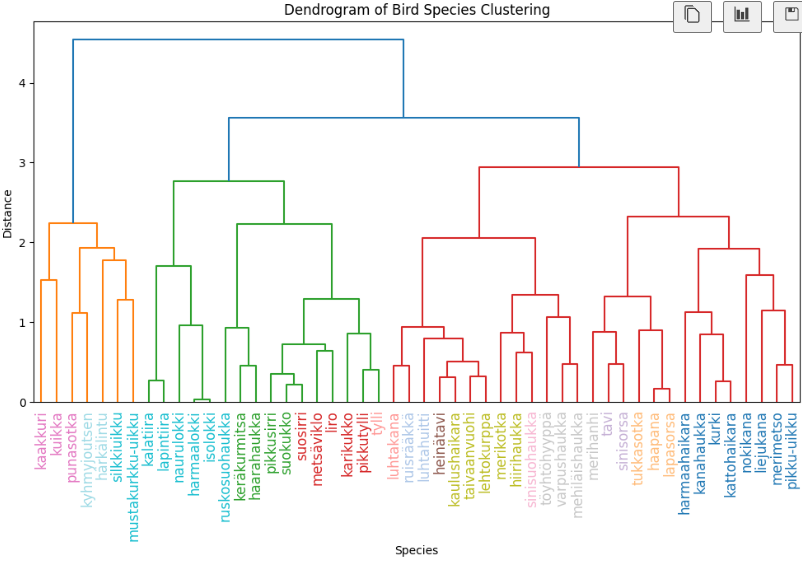
\includegraphics[width=0.8\textwidth,height=\textheight,keepaspectratio]
    {dendogram.png}
    \caption{\emph{Dendogram}}\label{fig:linkage-based dendogram}
\end{figure*}

\section{Conclusion}
Upon examination of the statistical properties, including \emph{min}, \emph{max},
\emph{mean}, \emph{variance}, and \emph{relative contrast}, it can be inferred
that the ``curse of dimensionality'' gives rise to unanticipated behaviors within
high-dimensional spaces. Specifically, the growth in dimensionality can yield
the following consequences:


\begin{itemize}
    \item Convergence of \emph{min}, \emph{mean}, and \emph{max} distances,
    causing the majority of data points to become equidistant.
    \item Decrease in \emph{variance} of distances, making distances of data
    points approach zero.
    \item Approach of \emph{relative contrast} towards zero, thereby
    diminishing the distinction between proximate and distant points.
\end{itemize}

In light of these observations, it becomes evident that the "curse of
dimensionality" poses significant challenges for certain machine learning
algorithms when operating in high-dimensional settings, thus necessitating 
appropriate adjustments to ensure optimal performance.


%Bibliography style. The alpha style generates references with 
%first letters and year. If you prefer numbers, use style plain.
% \bibliographystyle{alpha}
% \bibliographystyle{plain}
% \bibliography{ref}

% \printbibliography{}

% Demo for adding appendices
\begin{appendices}
    All code is publicly available on GitHub at \url{https://github.com/ancuongnguyen07/CS-E4650/tree/master/hw5}
\end{appendices}


\end{document}
